\documentclass[svgnames]{article}

\author{Eduard Scherer}
\title{Development \& Construction of an Autonomous Path-Following Drone}
\date{\today}
\usepackage[utf8]{inputenc}

\usepackage[
backend=biber,
style=numeric,
sorting=ynt
]{biblatex}
\addbibresource{references.bib} %Imports bibliography file

\usepackage{graphicx}
%\graphicspath{{C:\Users\eduar\Documents\Maturarbeit\MA-project\pictures}}

%imports parskip, which jumps to the next paragraph when pressing a double enter instead of doing \\
\usepackage{parskip}

\usepackage{color}
\definecolor{Blue}{rgb}{0,0,1}
\definecolor{Green}{rgb}{0,0.5,0}
\definecolor{Gray}{rgb}{0.5,0.5,0.5}
\definecolor{Fuchsia}{rgb}{1,0,1}

\usepackage{appendix}



\usepackage[dvipsnames,table,x11names]{xcolor}

% references for pictures



% imports tcolorbox
\usepackage{tcolorbox}
% adds a explanation box
\newtcolorbox[auto counter, number within=section]{Explanation}[2][]{%
	title=Explanation~\thetcbcounter: #1, colframe=blue!30, 
	coltitle= white}

\usepackage{amsmath}
\usepackage{array}




\makeglossary
\usepackage{lstautogobble}
\usepackage{listings}
\lstdefinestyle{BaselineStyle}
{ 
	commentstyle=\color{Blue},
	keywordstyle=\color{Green},
	numberstyle=\tiny\color{Gray},
	stringstyle=\color{Fuchsia},
	basicstyle=\ttfamily,
	columns=flexible,
	breakatwhitespace=false,
	breaklines=true,
	captionpos=b, % sets the caption position 
	keepspaces=true, % keeps spaces in text, keeping indentation of code
	keywordstyle=\color{blue},
	numbersep=5pt,
	showspaces=false,
	showstringspaces=false,
	showtabs=false,
	tabsize=2,
	% might be adding: stepnummer=2, to have only have every other line numbered
	xleftmargin=1.5em,
	frame=single,
	numbers=left,
	framexleftmargin=1.5em,
	autogobble=true
} 

% Python
\lstdefinestyle{myPython}
{ %
	language=Python,
	morekeywords={},
	backgroundcolor=\color{Pink!15},
	frame=none,
	framexleftmargin=0em,
	xleftmargin=0em,
	belowskip=0pt
} 

% set to 'BaselineStyle'
\lstset{style=BaselineStyle}

% imports glossaries and activates it
\usepackage[acronym, nomain]{glossaries}
\makeglossaries

\newacronym[plural={flight controllers (FCs)}]{Fc}{Fc}{flight controller}
\newacronym[plural={electronic speed controllers (ESCs)}]{ESC}{ESC}{electronic speed controller}
\newacronym{FPV}{FPV}{first person view}
\newacronym[plural=vertical takeoff and landing (VTOLs)]{VTOL}{VTOL}{vertical takeoff and landing}
\newacronym{GNSS}{GNSS}{global navigation satellite system}
\newacronym{GPS}{GPS}{global positioning system}
\newacronym{OS}{OS}{operating system}
\newacronym{SSH}{SSH}{secure shell}
\newacronym{DFU}{DFU}{device firmware updgrad}
\newacronym{PID}{PID}{proportional, integral, derivative}
\newacronym{AIO}{AIO}{All-in-One}
\newacronym{CEP}{CEP}{circular error probable}
\newacronym{LiPo}{LiPo}{lithium polymere}
\newacronym{Li-ion}{Li-ion}{lithium-ion}
\newacronym{VNC}{VNC}{virtual network computing}
\newacronym{venv}{venv}{virtual environment}
\newacronym{UAV}{UAV}{unmanned aerial vehicle}
\newacronym{OSS}{OSS}{open source software}
\newacronym[plural={printed circuit boards (PCBs)}]{PCB}{PCB}{printed circuit board}
\newacronym{RTCM}{RTCM}{radio technical commission for maritime}
\newacronym{RTK}{RTK}{real time kinematic}
\newacronym[plural=ground control stations (GCSs)]{GCS}{GCS}{ground control station}
\newacronym{MP}{MP}{Mission Planner}
\newacronym{UART}{UART}{universal asynchronous receiver/Transmitter}
\newacronym{bps}{bps}{bits per second}
\newacronym{I2C}{I2C}{inter-integrated circuit}
\newacronym{SDA}{SDA}{serial data}
\newacronym{SCL}{SCL}{serial clock}



\usepackage{hyperref}
\hypersetup{
	colorlinks,
	linkcolor={red!40!black},
	urlcolor={blue!90!black},
	citecolor=,
}
% Intelligent cross-referencing. [LOAD AFTER \hypersetup AND amsmath]
\usepackage[nameinlink,noabbrev,capitalise]{cleveref}


% Dokument
\begin{document}
\maketitle
\newpage
\tableofcontents
\newpage
% TODO link color really???
	\section{Introduction}
	
	In the today's where technology is advancing faster than ever before this Matura paper is enlightening the corner of self-built and autonomous drones.
	
	However, it first needs to be defined what a drone even is. According to the Cambridge Dictionary, a drone is defined as: \textit{an aircraft that does not have a pilot but is controlled by someone on the ground} \cite{cambridgedrone}. In this work, the term 'drone' will refer to a quadcopter which is a drone with four motors that lifts off and flies through the power provided by the motors and does not glide like a plane. There is also the term \gls{UAV}, however this is mostly used to describe military grade drones.

	In current conflicts the meanings of \gls{UAV} and quadcopters have become more entangled than ever. The typical hobbyist drone is now widely and effectively used to target enemy forces. In the Ukraine war drones are one of the most effective weapons to use against the Russian aggressor. For example, in this conflict drones are used with thermite canisters attached to them to target the enemies under tree covers \cite{thermitedrones}. Since the war began the drones have become increasingly autonomous. Drone pilots with more advanced setups, are able to simply lock onto the target and let the drone follow and detonate near it \cite{nytimesaidrones}. This increased use in war has also had an impact on the market for components. The most used \gls{ESC} firmware BLHeli\_32 ceased its operation due to laws being passed in Norway that penalised firms that are not able to verify that their products are not used in wars \cite{blhelidead}. However, this is really difficult to do regarding that the \glspl{ESC} are dual-use goods\footnote{Dual-use goods are products that are designed for civilian purposes, but in the wrong hands can become deadly weapons \cite{dualuse}.}.
	
%	Which is really difficult to do regarding that both sides in the Ukraine war are buying the \glspl{ESC} no matter what software is on them.  
	% Would have an additional article about drones that are produced in Switzerland that do the same thing
	
	The goal of this Matura paper is to develop an autonomous path-following drone, where path-following refers to navigating a \gls{GPS} path rather than following a ground path using image recognition. Additionally it should be written so that somebody with no prior knowledge about drones can read, easily understand, and also might reproduce the first part until \cref{companion computer} (Companion Computer). After that first part, having some understanding of python will be useful, but it is not a requirement. However, without prior knowledge, the explanations might be a bit confusing.

	I was first interested in drones when I was in fifth grade and got one as a Christmas present. After that, I also wrote a rather interesting piece about different types of drones in sixth grade, but I lost the interest shortly after. Later on, when I was in the "Gymnasium", I was randomly recommended a drone video on YouTube and began gaining interest again. I initially planned to build a \gls{FPV} drone. Sadly, I never really found the time to build one. When the Matura paper came around I found it to be the perfect opportunity to work with a drone. However, a \gls{FPV} can be bought as commodity in contrast to an autonomous drone. 
	% TODO something new


	\section{Literature Review}
	After extensive internet research it becomes clear that only one kind of a comparable published autonomous drone project exists, one with a \gls{Fc} from the Pixhawk family of \glspl{Fc} in connection to a RaspberryPi. However, it is clear that there are many underground drone laboratories in the Ukraine war, which do not publish their advances in drone technologies, due to the risk of being bomb by their own inventions. Additionally, there are many large firms, as Amazons, who are trying to deliver packages by drones \cite{amazondrone}.
	
	
	\section{Methodology}
	\subsection{General Software Considerations}

	\subsubsection{Open Source Software}
	The software integration in this Matura Paper is based on \gls{OSS}. \gls{OSS} is a software of which the source code is public. There is an important process known as 'forking', which refers to when a person other than the original developer takes the code and modifies it independently. The main benefit over closed software is that it can be freely downloaded by everyone and everybody can modify it as they see fit. However the downside is that if the development team loses interest, the software will become outdated and will not work smoothly with other systems anymore. Both aspects will later be found both useful and time-consuming. 
	% TODO question from the pdf about forking in the next section
	
	\subsubsection{Flight Softwares}
	Based on the literature reviewed there are three main software stacks to consider when it comes to drones: Betaflight, \myinav (\glsentrylong{INAV}), and Ardupilot. All of them are open source. Multiwii is the origin of Betaflight and \gls{INAV}. Multwii was Arduino based and then upgraded to Baseflight to be able to utilize a better chipset. Then it was forked to Cleanflight, which was later forked again into Betaflight and \gls{INAV} \cite{history}. 
	
	The following overview of the three softwares, is mostly based on the article written by \textcite{firmwarearticle} and a video made by \textcite{firmwarevideo}.
	
	Betaflight appears to be the go-to option for \gls{FPV}, commonly used for filming or racing. It is the most beginner friendly out of the three, because it has a large community, which results in a wide range of tutorials. When a new \gls{Fc} comes out it is normally made to be used with Betaflight. However, Betaflight lacks support for different types of vehicles and generally the automated features are less developed compared to the other two. 
	
	\gls{INAV} offers basic autonomous flight using waypoints and automated landing. It does not only support quadcopters, but also boats, rovers, planes and wings. It has a similar interface as Betaflight, so switching from one to the other is easier than switching from \gls{INAV} to Ardupilot.
	
	Ardupilot basically offers everything the other two have to offer and more, for example Submarines and \glspl{VTOL}. Although it is not commonly used with \gls{FPV}, it is still possible. Ardupilot involves more steps to set up, which also leads to the main benefit of it, namely the nearly limitless customization options.

	
	It is also the only option to use together with a companion computer like the RaspberryPi. A few years ago it was really expensive to start, because it only supported the Pixhawk family of flight controllers which cost a few hundred Francs per piece. However, in recent years it has began to support more and cheaper flight controllers.
	


	\subsection{Drone Overview}
	If you want to fly a drone you have two options available: either you buy one or you build one. From a technical viewpoint, the second option is, not only the better option but also the cheaper one. Additionally, in the case of this Matura paper there is not an option to buy a prebuilt drone. 
	% TODO not as standard existing not an option does not exist compared to \gls{FPV} which xould be bought prebuilt
	
	The main parts needed for a drone are the \gls{Fc}, the \gls{ESC}, the receiver, the battery, servos and of course the mainframe. Additionally a \gls{GPS} and LEDs can be added as needed. The \gls{Fc} and the \gls{ESC} are sometimes more generally referred to as \glspl{PCB}\footnote{A \gls{PCB} is a flat board that houses electronic components and features conductive pathways etched onto its surface to connect those components.} or simply 'boards'.


	The \gls{Fc} runs the chosen software and controls every other part in one way or another. It is directly connected to the \gls{ESC}, which controls the motors and is connected to the battery. The \gls{Fc} also communicates with the receiver and, if present, the \gls{GPS}. In this case there will also be a microcomputer, I chose the RaspberryPi, which connects to the \gls{Fc}. The connections between the parts are shown in \cref{fig:cheappartconnection}.
	\begin{figure}
		\centering
		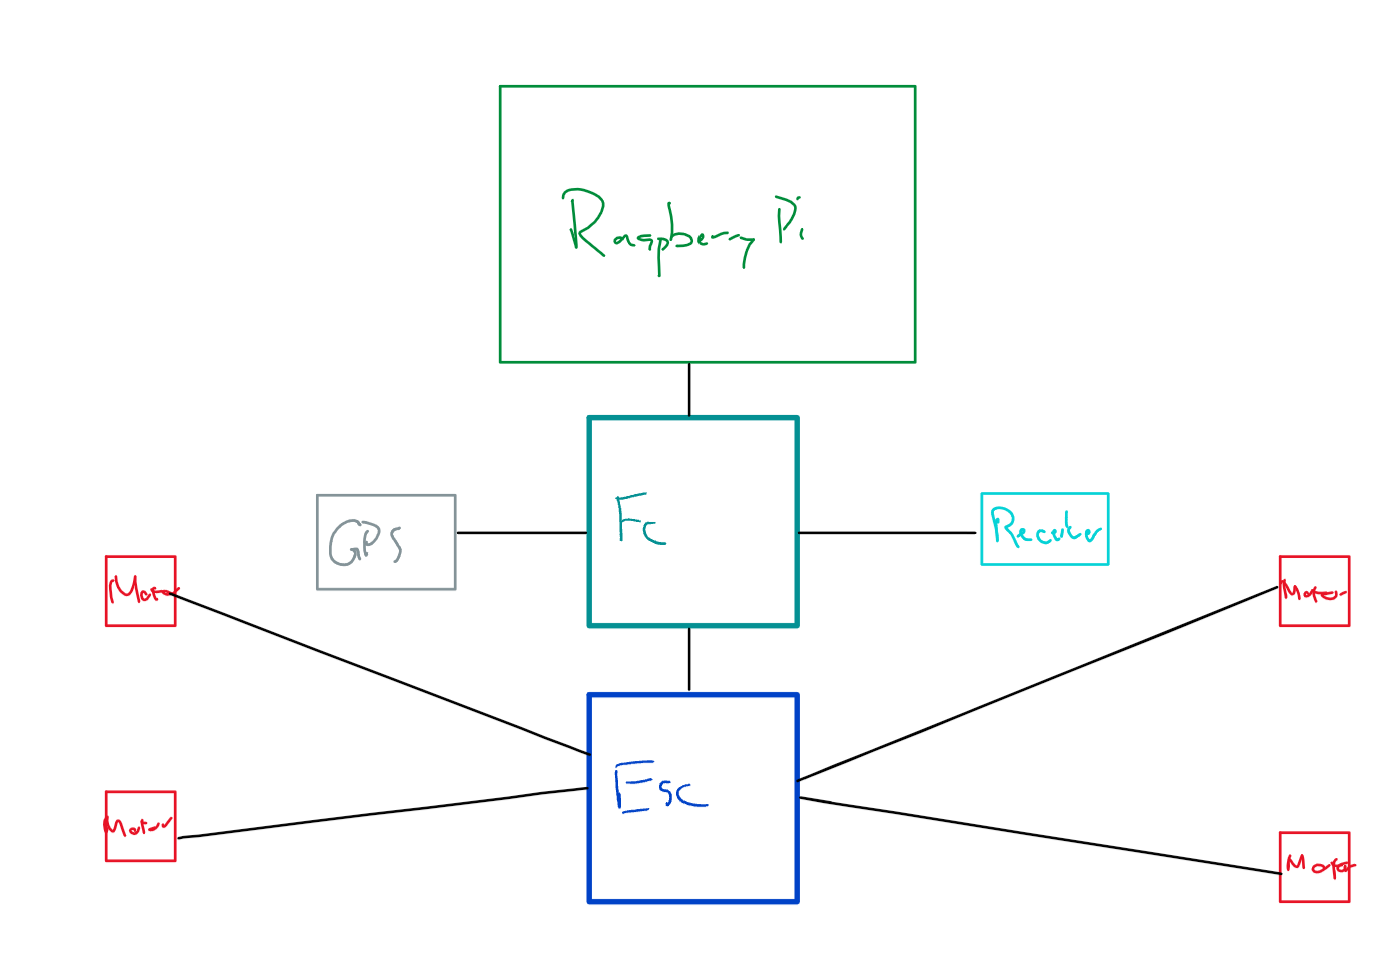
\includegraphics[width=0.7\linewidth]{pictures/cheappartconnection}
		\caption{connection between the parts}
		\label{fig:cheappartconnection}
	\end{figure} 
	% TODO do the numbers to reference data changes, already in the connection sketch
	
	% TODO add a graphic which illustrates the connection between the parts
	
	\subsection{Data Transfer Protocols}
	There are two types of data transfer protocols: serial and parallel. The way they transfer data is by pulsing 5V for a 1 and 0V for a 0. The difference is that the parallel communication sends the data for each bit parallel to the other 7 bits through eight connections, as seen in \cref{parallel}, and the serial sends the data over one connection. This also requires a clock to synchronize the output of data.
	% TODO order the picture somewhat smartly
	\begin{figure}[ht]
		\centering
		\begin{minipage}[c]{0.4\textwidth}
			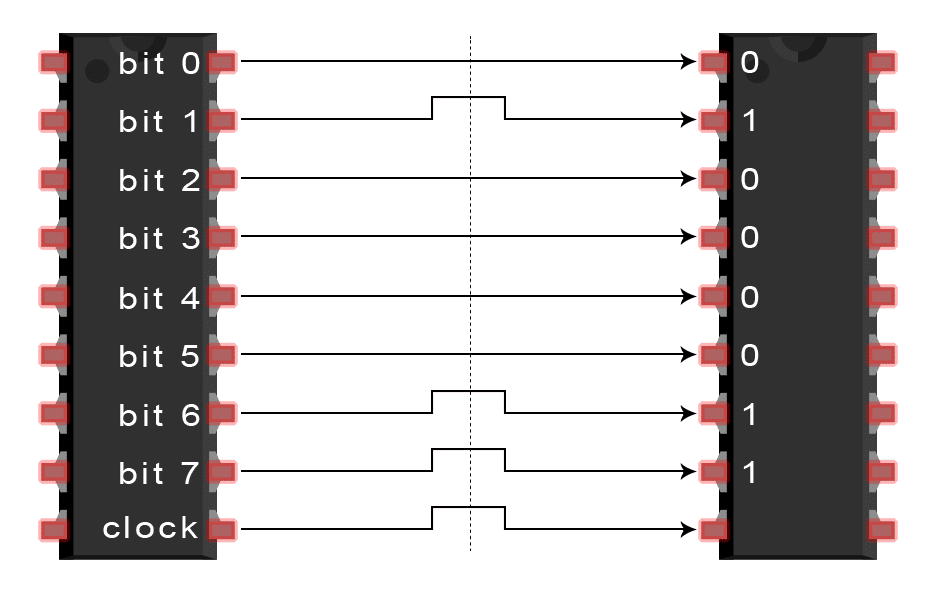
\includegraphics[width=\textwidth]{pictures/SPIparallel}
			\caption{parallel communication of the letter "C" \cite{spiprotocol}}
			\label{parallel}
		\end{minipage}
		\hfill
		\begin{minipage}[c]{0.4\textwidth}
			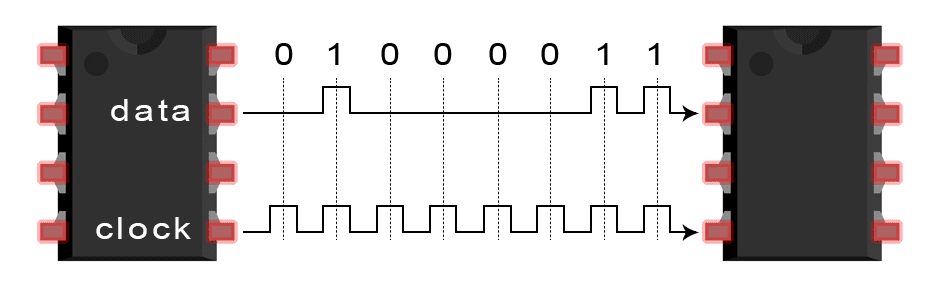
\includegraphics[width=\textwidth]{pictures/SPIserial}
			\caption{serial communication of the letter "C" \cite{spiprotocol}}
			\label{serial}
		\end{minipage}
	\end{figure}
	
	\subsubsection{Uart}
	The \gls{UART} is a physical circuit \cite{uartprotocol}. In the field of self-built drones it is used to communicate to and from the \gls{Fc}. It works by transmitting data asynchronously. Instead it has a so-called baud rate, which is a measure of \gls{bps}. When connecting two \gls{UART} microcontrollers there are two lines needed from the Tx of one to the Rx of the other and vice versa, as shown in \cref{fig:uartconnection}. With a \gls{UART} a data packet is transferred instead of individual bits. The packet consists of a start bit, followed by 5 to 9 data bits and at the end there are 1 to 2 stop bits, as shown in \cref{fig:uartpackage}. There is also the option to include a parity bit instead of one of the data bits. A parity bit is used to verify that none of the bits were changed during the transfer. It is a 0 if the number of 1 in the sequence is even and 1 if it is odd.
	% TODO reference control
\begin{figure}[ht]
	\begin{minipage}[c]{0.4\textwidth}
		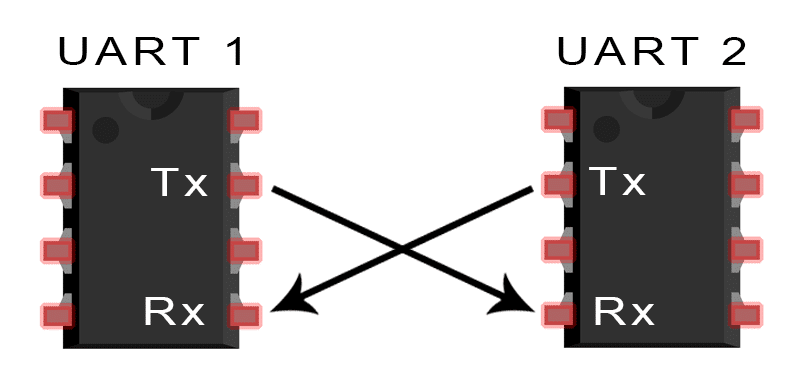
\includegraphics[width=\textwidth]{pictures/UARTconnection}
		\caption{\gls{UART} connection \cite{uartprotocol}}
		\label{fig:uartconnection}
	\end{minipage}
	\hfill
	\begin{minipage}[c]{0.4\textwidth}
		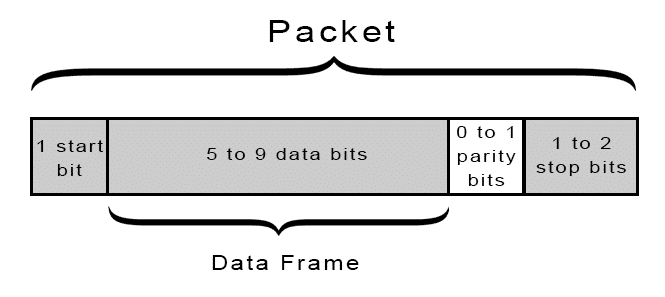
\includegraphics[width=\textwidth]{pictures/Uartpackage}
		\caption{\gls{UART} packet \cite{uartprotocol}}
		\label{fig:uartpackage}
	\end{minipage}
	
\end{figure}

	\subsubsection{I2C}
	The \gls{I2C} communication is also serial like \gls{UART}, but it has the advantage of being able to communicate to more than one slave\footnote{The relationship between two parts where one controls the other is called a master-slave relationship \cite{i2cprotocol}. Obviously the master is the one that controls the slave. Although the terminology is rather controversial, it is still widely used \cite{masterslave}.} part. In this work, it is used for the compass built into the \gls{GPS}. There are two lines between the master and the slave; the \gls{SDA} and the \gls{SCL}. The \gls{SCL} line is used for synchronization and the \gls{SDA} line for the transfer of a packet. The data packet looks quite different to the one from the \gls{UART}. There is a start condition, afterwards the address frame is used to figure out to which slave the packet goes, followed by a bit to determine if the master sends or requests data, the data is followed by a ACK/NACK\footnote{ACK stands for acknowledgment and NACK for negative acknowledgment} bit, which confirms either that the data frame was received or not, and at the end there is a stop condition.
\begin{figure}[ht]
	\begin{minipage}[c]{0.4\textwidth}
		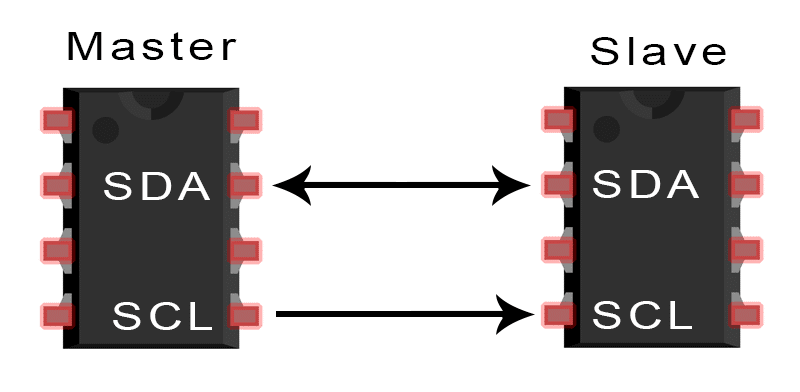
\includegraphics[width=\textwidth]{pictures/I2Cconnection}
		\caption{\gls{I2C} connection \cite{i2cprotocol}}
		\label{fig:I2Cconnection}
	\end{minipage}
	\hfill
	\begin{minipage}[c]{0.4\textwidth}
		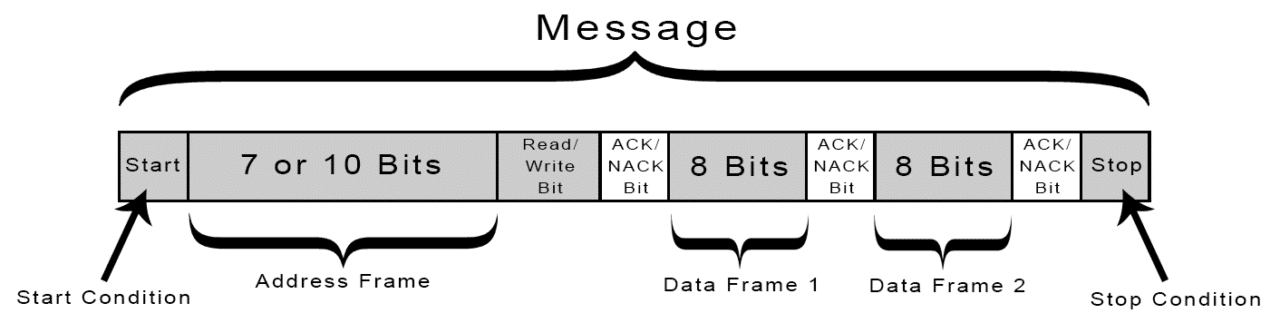
\includegraphics[width=\textwidth]{pictures/I2Cpackage}
		\caption{\gls{I2C} package \cite{i2cprotocol}}
		\label{fig:I2Cpackage}
	\end{minipage}
\end{figure}

% TODO make figure on the left larger cannot read do only after decreasing the space on the sid, top and bottom
	\subsubsection{MAVLink}
	The MAVLink protocol is more complex compared to \gls{UART} or \gls{I2C}. It can transfer up to 263 bytes or 280 bytes, depending on the version used. It is used for the connection between the \gls{Fc} and a \gls{GCS} or in this case the RaspberryPi companion computer.
	\subsection{Parts}
	
	\subsubsection[Fc]{Flight Controller}
	There are two different types of flight controllers: the \gls{AIO} and a standalone \gls{Fc}. The \gls{AIO} consists not only a \gls{Fc} but also the \gls{ESC} on the same board. This has the advantage of only needing one board instead of two or five, in some alternative setups. However, if only parts of the \gls{ESC} or the \gls{Fc} are damaged you need to replace the whole board, which is more expensive than replacing only the \gls{Fc} or \gls{ESC}. 
	
	Betaflight and \gls{INAV} both support a wide variety of \glspl{Fc} compared to Ardupilot which is only supporting a very specific sample of boards \cite{FcSupport}. They have the option of open and closed hardware. Because the open hardware \glspl{Fc} are quite expensive. This is why I decided to go with a closed one. The chip used in \glspl{Fc} is usually a STM32. There are multiple generations of it the mainly used ones are F4, F7 and H7, the newest version is the H7. I then decided to go with the Kakute H7 v1.3 (MPU6000) from Holybro, because it was affordable and available as a stack \cite{KakuteH7}. A stack is a \gls{Fc} and \gls{ESC} mounted on top of each other. It normally comes with stack screws. It is shipped with Betaflight so it is required to flash Ardupilot. 
	\begin{Explanation}[open and closed hardware]
		\item Like open source software, the "source code" -or in this case blueprints- open hardware can be accessed by everyone and adjusted to meet one's individual needs \cite{openhardware}.
	\end{Explanation}




	\subsubsection[ESC]{Electronic Speed Controler}
	There are two different kind of \gls{ESC}s: 4in1 and single \glspl{ESC}. If you use single \gls{ESC}s, then one is needed for each motor instead of a single board for all of them. The advantage of 4in1 \gls{ESC}s is that it does not require a power distribution board, because it is already incorporated in the \gls{ESC}, and that it can come in a stack. The disadvantage is that if a part of the \gls{ESC} is damaged you need to replace the whole board. What needs to be considered before buying a \gls{ESC} is that the peak current of the motor is not higher than the burst current of the \gls{ESC}, because a too high current could damage the \gls{ESC}.
	
	My decision was to go with a 4in1 on a stack, because it is slightly cheaper and normally easier to wire compared to four single boards. The only option with the Kakute H7 was the stack with the Tekko32 4in1 with a continuous current of either 50A, 60A or 65A. I chose the 50A one, because you do not need a high continuous current rating when flying rather slowly and the motors I chose have a peak current of around 42A \cite{Tekko32}. 
	
	At the time I bought the Tekko32, it was still shipped with BLHeli32, which as mentioned in the beginning has since seized their operations. It is however possible to flash AM32\footnote{A different \gls{ESC} software, which has gained quite some popularity after BLHeli32 is off the market.} onto it \cite{AM32}.

	\subsubsection{Motor}
	There are two types of motors: brushed and brushless ones. Brushed motors are used in very small drones with 1S\footnote{What 1S means will be explained in the next section} batteries. However, even in smaller drones brushless motors are the more popular choice \cite{brush/lessmotors}. A brushed motor, as shown on the left in \cref{fig:brushedbrushlessmotor}, works by having two brushes that are delivering the power to a coil in the middle of a permanent magnet. This creates a magnetic field around the coiled, which is then attracted to the magnet surrounding it. Due to the commutator the direction in which the provided electricity flows is changed every half turn. This causes the magnetic field around the coil to change the direction and in turn gets attracted to the other side of the magnet. A brushless motor, as shown in \cref{fig:brushedbrushlessmotor} on the right, works by having a field magnet in the middle and coils surrounding it. The coils surrounding the magnet are part of the so-called stator. These coils are provided with a positive and negative voltage, which will cause the magnetic field around them to alternate. When the alternation is synchronized, which is done by an \gls{ESC}, it will cause the field magnet to spin. 
\begin{figure}[ht]
	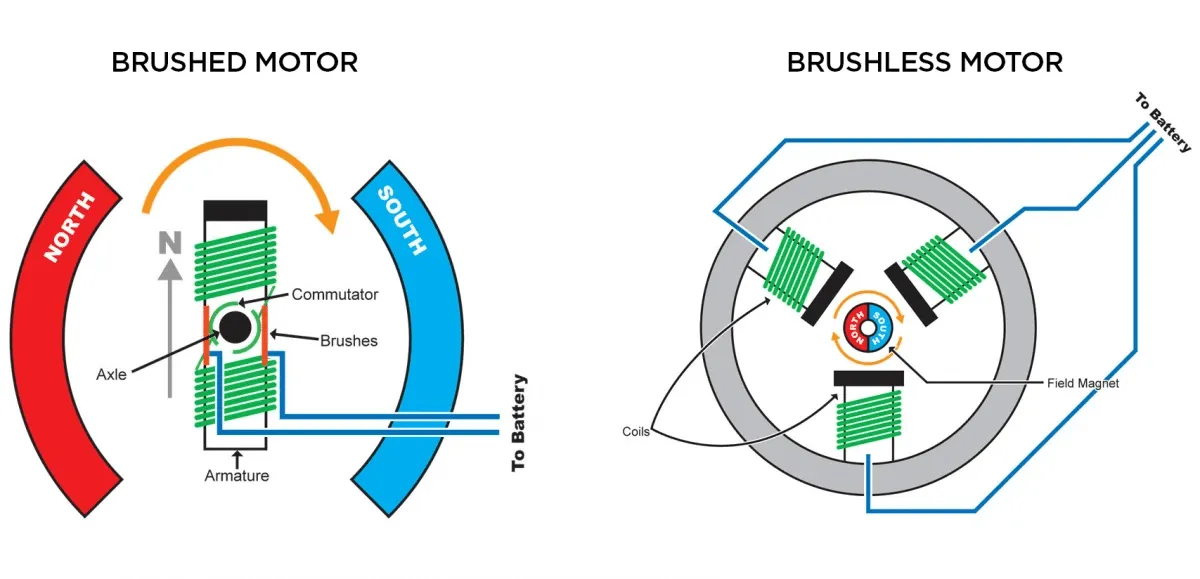
\includegraphics[width=0.9\columnwidth]{pictures/brushed_brushlessmotor}
	\caption{brushed and brushless motors \cite{brushlessedmotor}}
	\label{fig:brushedbrushlessmotor}
\end{figure}

	The numbers that are seen on the motors, such as '2207', describe the stator of the motor itself. In the case of a 2207 that would be a 22mm diameter and a height of 7mm. The usual stator sizes of 5 inch drones are either 2207 or 2306. There is also the KV value, which has to be considered. The KV value is the number of revolutions per minute (rpm) a motor turns when one volt is applied. The lower the KV value, the more efficient the motor is and the higher the KV value the more responsive it is. The KV value for a 5-inch drone with a 4S battery ranges from 2300 to 2800. I chose the Iflight Xing-E Pro 2207\cite{xingepro} with a KV value of 2450, because the IFlight-Xing motors are known to be of good quality, \textit{'they (Xing motors) also prove to be very reliable and most importantly durable'} \textcite{xingreview}. 


	
	\subsubsection{Battery}
	There are two main types of batteries: \gls{LiPo} and \gls{Li-ion} batteries. \gls{LiPo} batteries have a tendency to go up in flames. They have a much higher discharge rate compared to \gls{Li-ion} batteries, also denoted as the C value, so they are well suited for racing drones. However, \gls{Li-ion} batteries have a higher energy density, which means that they can store more mAh for the same weight compared to \gls{LiPo} batteries, so they are more common in long-range flying. The batteries normally have multiple cells, for example a 4S \gls{LiPo} battery contains 4 cells. This is important, because the more cells you have, the higher is the voltage and so you will need a motor with a lower KV value. 
	 
	I first wanted to buy two \gls{Li-ion} battery packs, however they are hard to get and much more expensive. The other option would be to solder them together in parallel, but it requires some soldering skill, which I personally did not have at the time. Hence I decided to go with 4S \gls{LiPo} batteries from the Tattu R-line with 120C and 2000mAh, because it needs to also power the RaspberryPi and testing the drone is rather tedious, when one needs to go back to charge every few minutes \cite{tattu}. I chose the brand Tattu, because it was the only known brand that was on AliExpress, from where I also sourced all the other components, so it seemed to be easier to also chose a battery from there. 

	\subsubsection{GNSS(Global Navigation Satellite System)/Compass}
	There are two different kinds of \gls{GNSS}\footnote{The \gls{GNSS} is usually referred to as \gls{GPS} even though \gls{GPS} is only the American \gls{GNSS} system} modules: the normal \gls{GPS} and compass boards and \gls{RTK} \gls{GPS}. Usually the chips used in both the RTK GPS and the normal GPS are manufactured by the company Ublox. The RTK GPS can achieve an accuracy of 1cm by incorporating information correction data from a \gls{RTCM}\footnote{It was first used for the positions of boats and other maritime vessels}. However, the correction data is either subscription-based, not guaranteed to cover all of the area or one needs to build one by themselves, which is quite complicated \cite{rtkgps}. For a small drone it may not be worth it to have a \gls{RTK} \gls{GPS} that costs several hundred Swiss Franks instead of a \gls{GPS} with a 2m \gls{CEP} which costs less than 30 Swiss Franks. Some of the \gls{GPS} units also have a compass built-in, so you will not need to buy an extra compass when using ArduPilot. 
	\begin{Explanation}[circular error probable (CEP)]
		\item The \gls{CEP} refers to how close to the real value the \gls{GPS} normally is. So if a \gls{GPS} has a \gls{CEP}
		of 2m it is normally in the range of 2 meters of the correct value \cite{CEP}.
	\end{Explanation}
	
	I chose the Holybro Micro M10 \gls{GPS}, because it is produced by the same brand as the Fc and therefore seemed to be easier to connect \cite{holybrom10micro}. In addition, the M10 chip is the newest version of Ublox chips and it would be pointless to buy an older version at the same price. It also is at least as good as other better-known GPS as the Matek M10Q \cite{gpstest} and comes with a built-in compass that is needed for ArduPilot.

	\subsubsection{Radio/Transmitter}
	The following information about transmitter protocols is based on two YouTube videos from \textcite{transprotocols} and \textcite{mlrs}.
	
	The two things to consider when it comes to transmitter protocols are latency and range. Latency is the delay between the input of the radio controller and when the \gls{Fc} reacts. The lower the latency, the faster the drone will react, to the inputs from the radiocontroler. It is related to the frequency bands of the receiver, of which there are normally two: 900 MHz and 2.4 GHz. When both are optimized the 900 MHz has better penetration and range, due to the longer wavelength, while the 2.4 GHz has a higher latency, because the frequency allows for faster data transmission.

	\subsubsection*{ExpressLRS\protect\footnote{The LRS stands for long range system.}}
	ExpressLRS is the best protocol in long range and for the combination of long range and low latency. It has been shown by \textcite{elrswezley}\footnote{Due to him being fined by the Australian government he took down his own video, so only a copy from an other YouTube channel exists.} that it really can fly up to 100km away from the starting point. There are two version: a 900 MHz and a 2.4 GHz. The main difference is that the 2.4 GHz can reach over 30km, but it is unlikely to go to 100km. However, it has the lowest latency. It is together with mLRS the only protocol that is open-source.
	% TODO at the end check if this footnote still references the one from ExpressLRS
	\subsubsection*{mLRS\protect\footnote[9]{}}
	The main difference between ExpressLRS and mLRS is that mLRS has a higher latency, which allows it to send larger data packages to your telemetry device. Which is something that is needed if you want to adjust something or get more data from your drone over the MAVLink protocol during the flight. 
	
	\subsubsection*{Transmitter/Radio}
	I decided to go with the Radiomaster RP4TD ExpressLRS 2.4GHz True Diversity Receiver based on a recommendation of a friend \cite{radiomasterreceiver}. It is also compatible with mLRS if I want to switch later on.
	
	I chose with the Radiomaster Boxer radio, because it is somewhat in the middle range from radios and seems to be quite reliable and has many switches to assign flight modes or other functions too  \cite{radiomasterboxer}. 

	\subsubsection{Smoke Stopper}
	A smoke stopper is a device that prevents the ESC from short-circuiting due to incorrectly soldered parts and can save quite a lot of money. There are two groups of smoke stoppers one that you buy and get destroyed when the ESC short circuits instead of the ESC. There is another category that does not destroy itself and there are also some that you can solder together on your own \cite{smokestopper}. 
	
	\subsubsection{Propellers and Battery Charger}
	For the propellers and battery chargers, I went off the recommendations from AOS-RC and FPVknowitall. I chose the Foxeer Donut 5145  and the HQ 5x4.3x3 V1S \cite{toroidal, hqprops}. For the battery charger, I went with the cheapest option the 608 AC Lipo Battery Charger \cite{lipocharger}.


	\subsubsection{Problems with the Parts Procurement}
	There were mainly two problems that. One less severe than the other. The first problem was that my ordered Kakute-Tekko stack did not include stack screws, which they normally do. Stack screws are just screws that you can use to mount the stack onto the frame. So I needed to purchase them separately, which was rather tedious and time-consuming.
	
	The more severe problem I ran into was that the batteries from AliExpress were first withheld by the Swiss border control and then I received two insect traps instead of batteries. Luckily I ordered one of the same batteries from another online shop (Conrad), because the other two took too long to deliver.
	
	Two months later, when my father decided to open the insect traps. To our surprise, the LiPo batteries were inside the insect traps at the bottom. And in hindsight it was also obvious that they were in there, because it had the numbering 3 4s 2000 on top which stands for version 3 of the 4s batteries with 2000 mAh. However, we dismissed the numbering on top as just some random numbers put there. 
	

	\subsection{ArduPilot}
	This chapter summarizes everything done for the first time flying and what could go wrong based on my experience. It is based on the ArduPilot copter documentation \cite{ardupilotdocs}.
	
	\subsubsection{Ground Station}
	To configure ArduPilot, there are multiple softwares, so called \gls{GCS} required. Usually they are ground-based and can transmit data via wireless telemetry device or USB cable.  With the telemetry device, they are able to control the drone from the ground and alter the route as the drone is autonomously flying. 
	
	The most widely used \gls{GCS} is \gls{MP}, but runs only on Windows and Mac OS. It has a wiki, which was used for the first-time configuration of my drone \cite{MissionPlanner}. 
	
	Another \gls{GCS} is MavProxy. It is written in python and intended to be used on Unix-based systems. MavProxy will be used to test the connection between the \gls{Fc} and the RaspberryPi, which is using the Debian \gls{OS}, a Unix-based system.
	\begin{Explanation}[operating system(OS)]
		\item A \gls{OS} is a software, which controls all the hardware of a computer.
	\end{Explanation}

	\subsubsection{Firmware Installation}
	The following section until \cref{companion computer} (Companion Computer) is rather technical and contains the necessary information for the steps to reproduce my setup.
	
	For the first time installation, the Kakute H7 is required to be flashed with ArduPilot, because it is shipped with Betaflight. 
	\begin{Explanation}[to flash]
		\item Flashing is the process of taking new firmware and loading it onto the device the firmware is needed on.
	\end{Explanation} 
	To install the ArduPilot firmware on the Kakute H7  it needs to be downloaded onto a computer \cite{ArduPilotFirmware}. Afterwards the STM32CubeProgrammer is used to flash the firmware onto the Fc \cite{STM32CubeProgrammer}. The \gls{Fc} in \gls{DFU} mode is directly connected with the computer, using a USB cable. Then the USB port, with which the \gls{Fc} is connected, is select and firmware is flashed onto the \gls{Fc} . A reboot is required to leave the \gls{DFU} mode, before connecting the \gls{Fc} to \gls{MP}. The progress of flashing the firmware was straightforward, unlike the rest of the configuration.

	
	\begin{Explanation}[device firmware upgrade (DFU)]% no \gls because it looks bad in the text box
		\item The \gls{DFU} mode is the mode, which allows the user to upload new firmware to the \gls{Fc}. It is normally accessible through a button which needs to be pressed, while connecting the battery. 
	\end{Explanation}


	\subsubsection{GPS Connection}
	In the beginning no immediate \gls{GPS} connection appeared. Even changing the parameter \lstinline|GPS_Type = 2| for the Ublox \gls{GPS}, the 'No \gls{GPS}' error, as seen in the bottom right corner of \cref{fig:nogps}, still occurred. Even though it was clear the \gls{GPS} was working and connected to the \gls{Fc}, because the compass, which is part of the \gls{GPS}, appeared in \gls{MP} and the \gls{GPS} blinked blue, indicating a connection to a \gls{GNSS}.
\begin{figure}[ht]
	\centering
	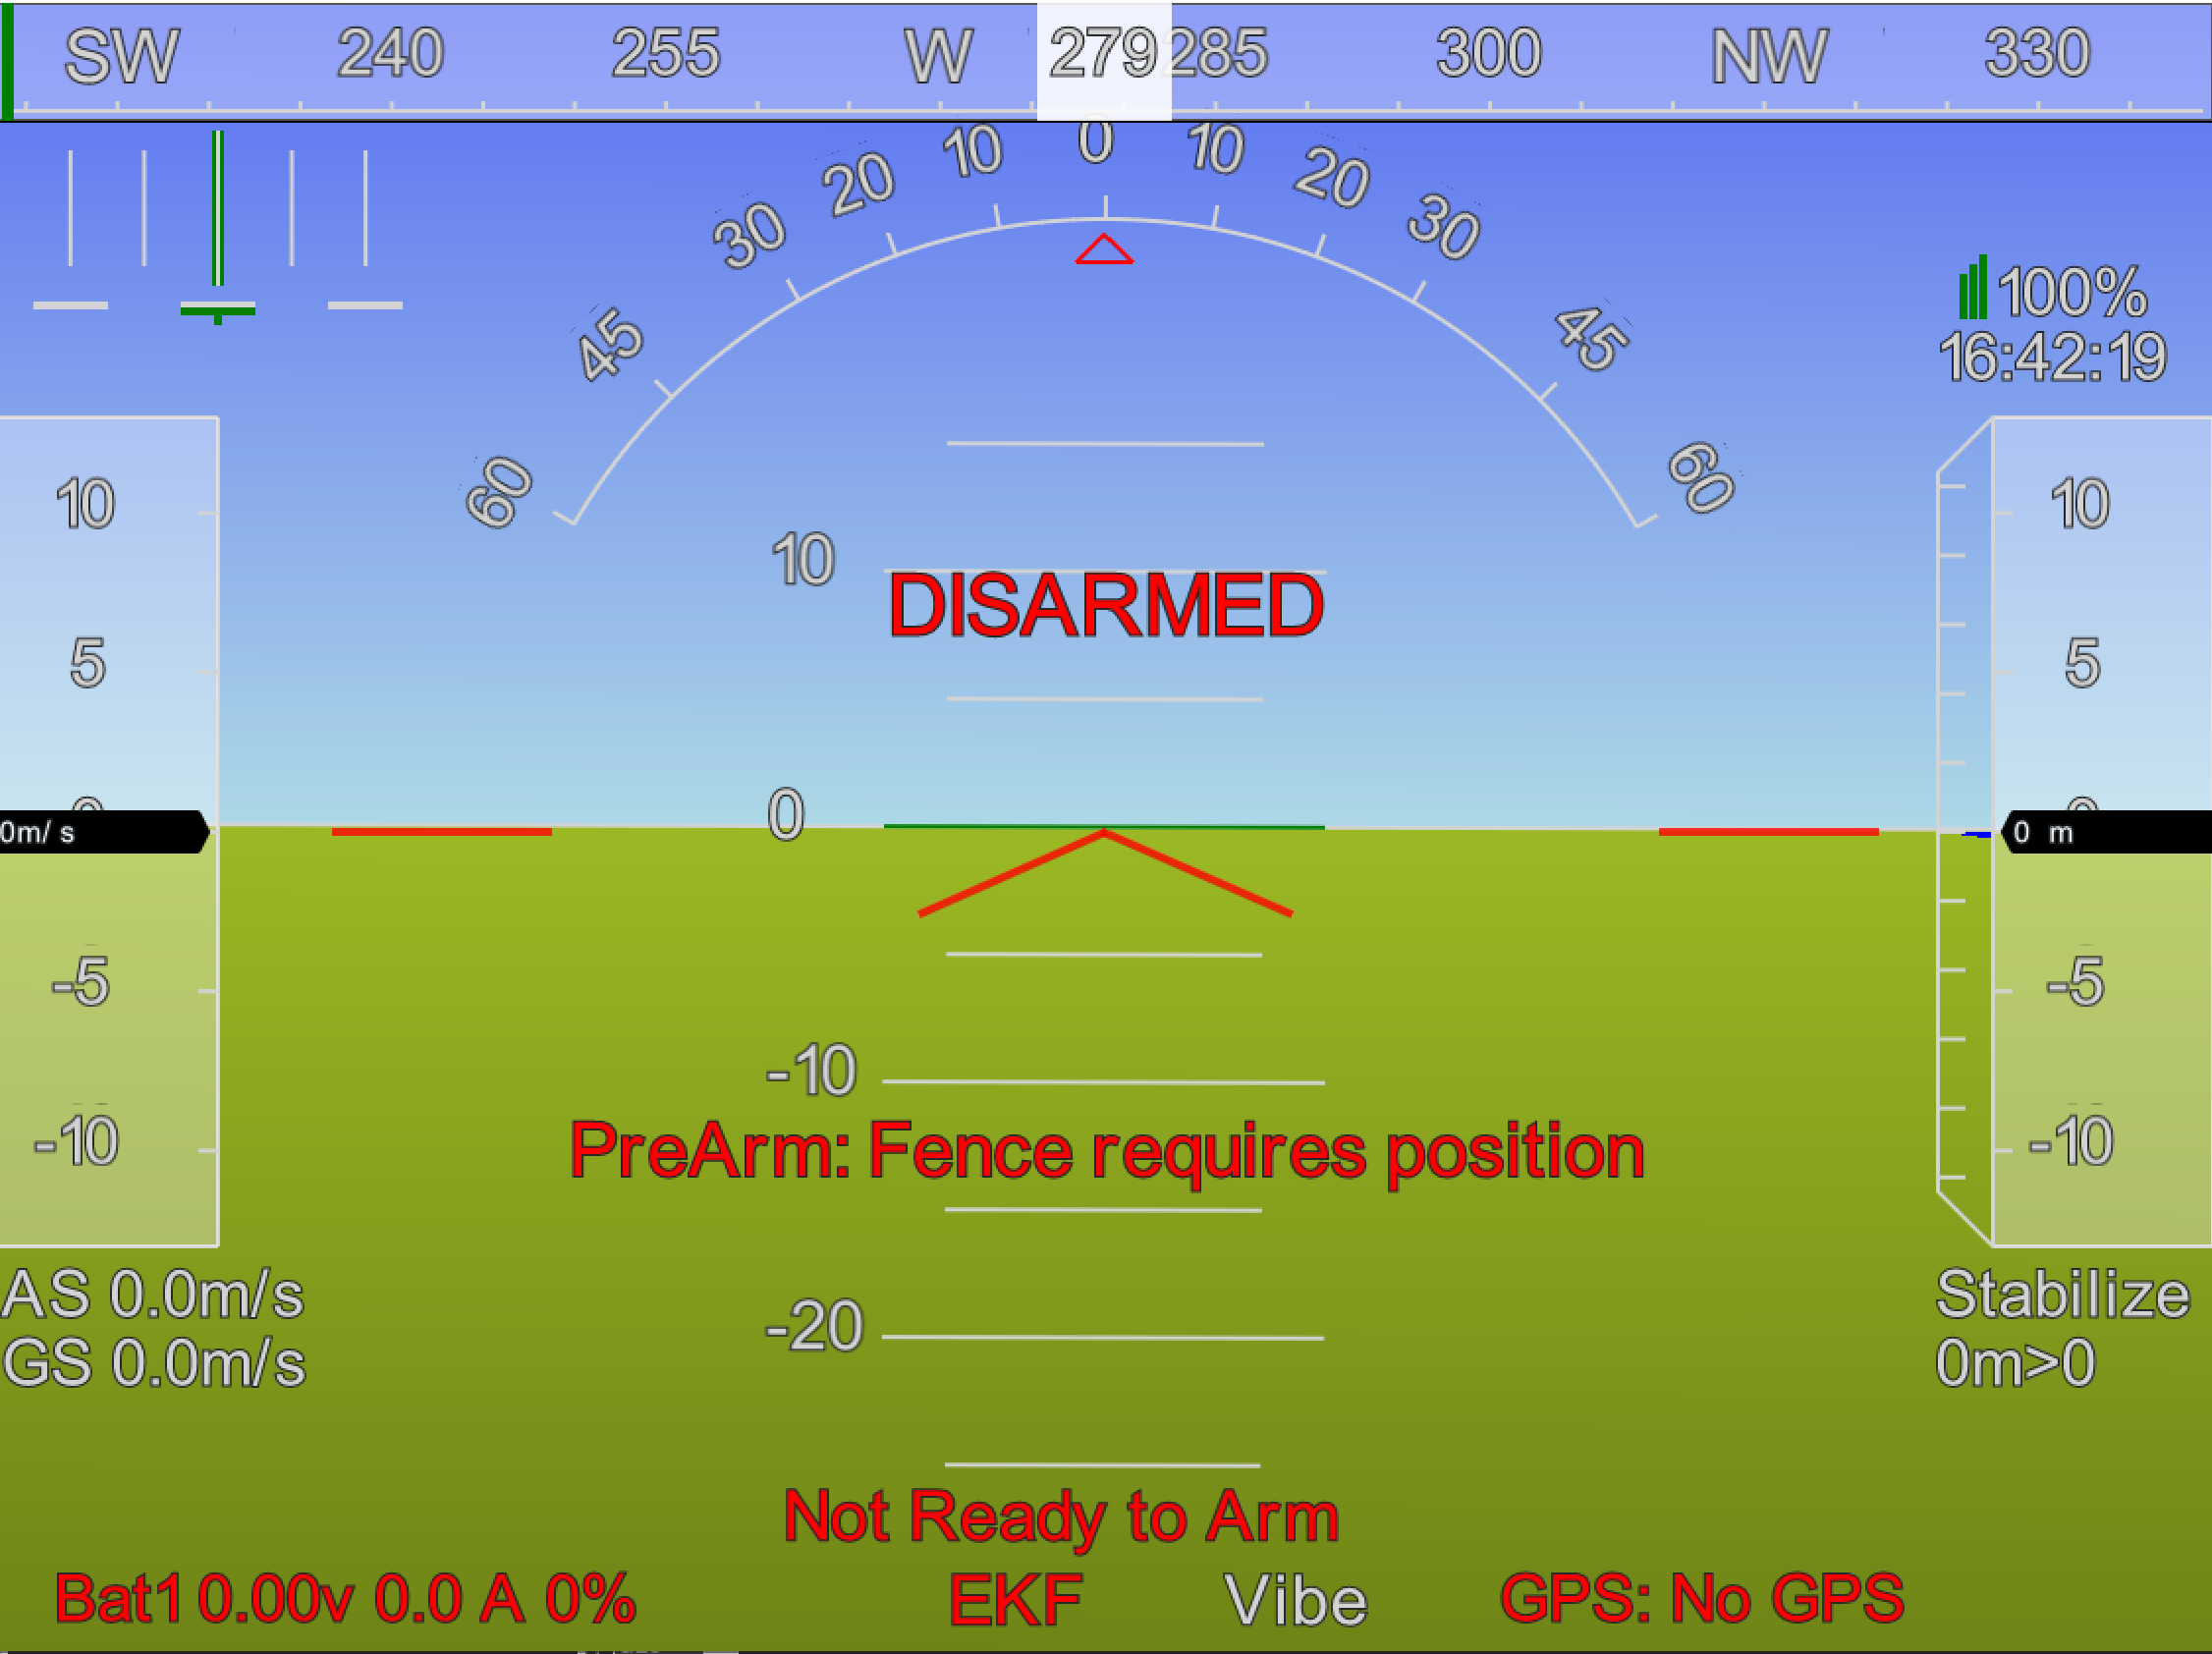
\includegraphics[scale=0.2]{pictures/No_GPS}
	\caption{No \gls{GPS} connection}
	\label{fig:nogps}
\end{figure}

	The issue could be that the \gls{GPS} is too close to metal surfaces, the computer, which is connected via USB cable, is too close, or that soldering was done poorly and the cables from the \gls{GPS} to the \gls{Fc} are falsely connected. After testing for each of the possible issues and mitigating the proximity in which metal was near the drone, the \gls{GPS} was still not working.

	The problem was that the \lstinline|Serial3_Protocol| (which is for the Uart3 that will be used for the connection to the RaspberryPi) was set to 5 which stands for \gls{GPS}. However, this blocked the Uart4 from being received as a \gls{GPS}, to which the \gls{GPS} was connected. After disabling Uart3 it finally worked.
	% TODO how did I find this out

	The GPS is quite precise outside \cref{fig:gpsoutside}\footnote{It sometimes works inside and is precisely on my room, but it might also show that it is in Poland, the middle of the Atlantic Ocean, or Iceland.}.
	
\begin{figure}[ht]
	\centering
	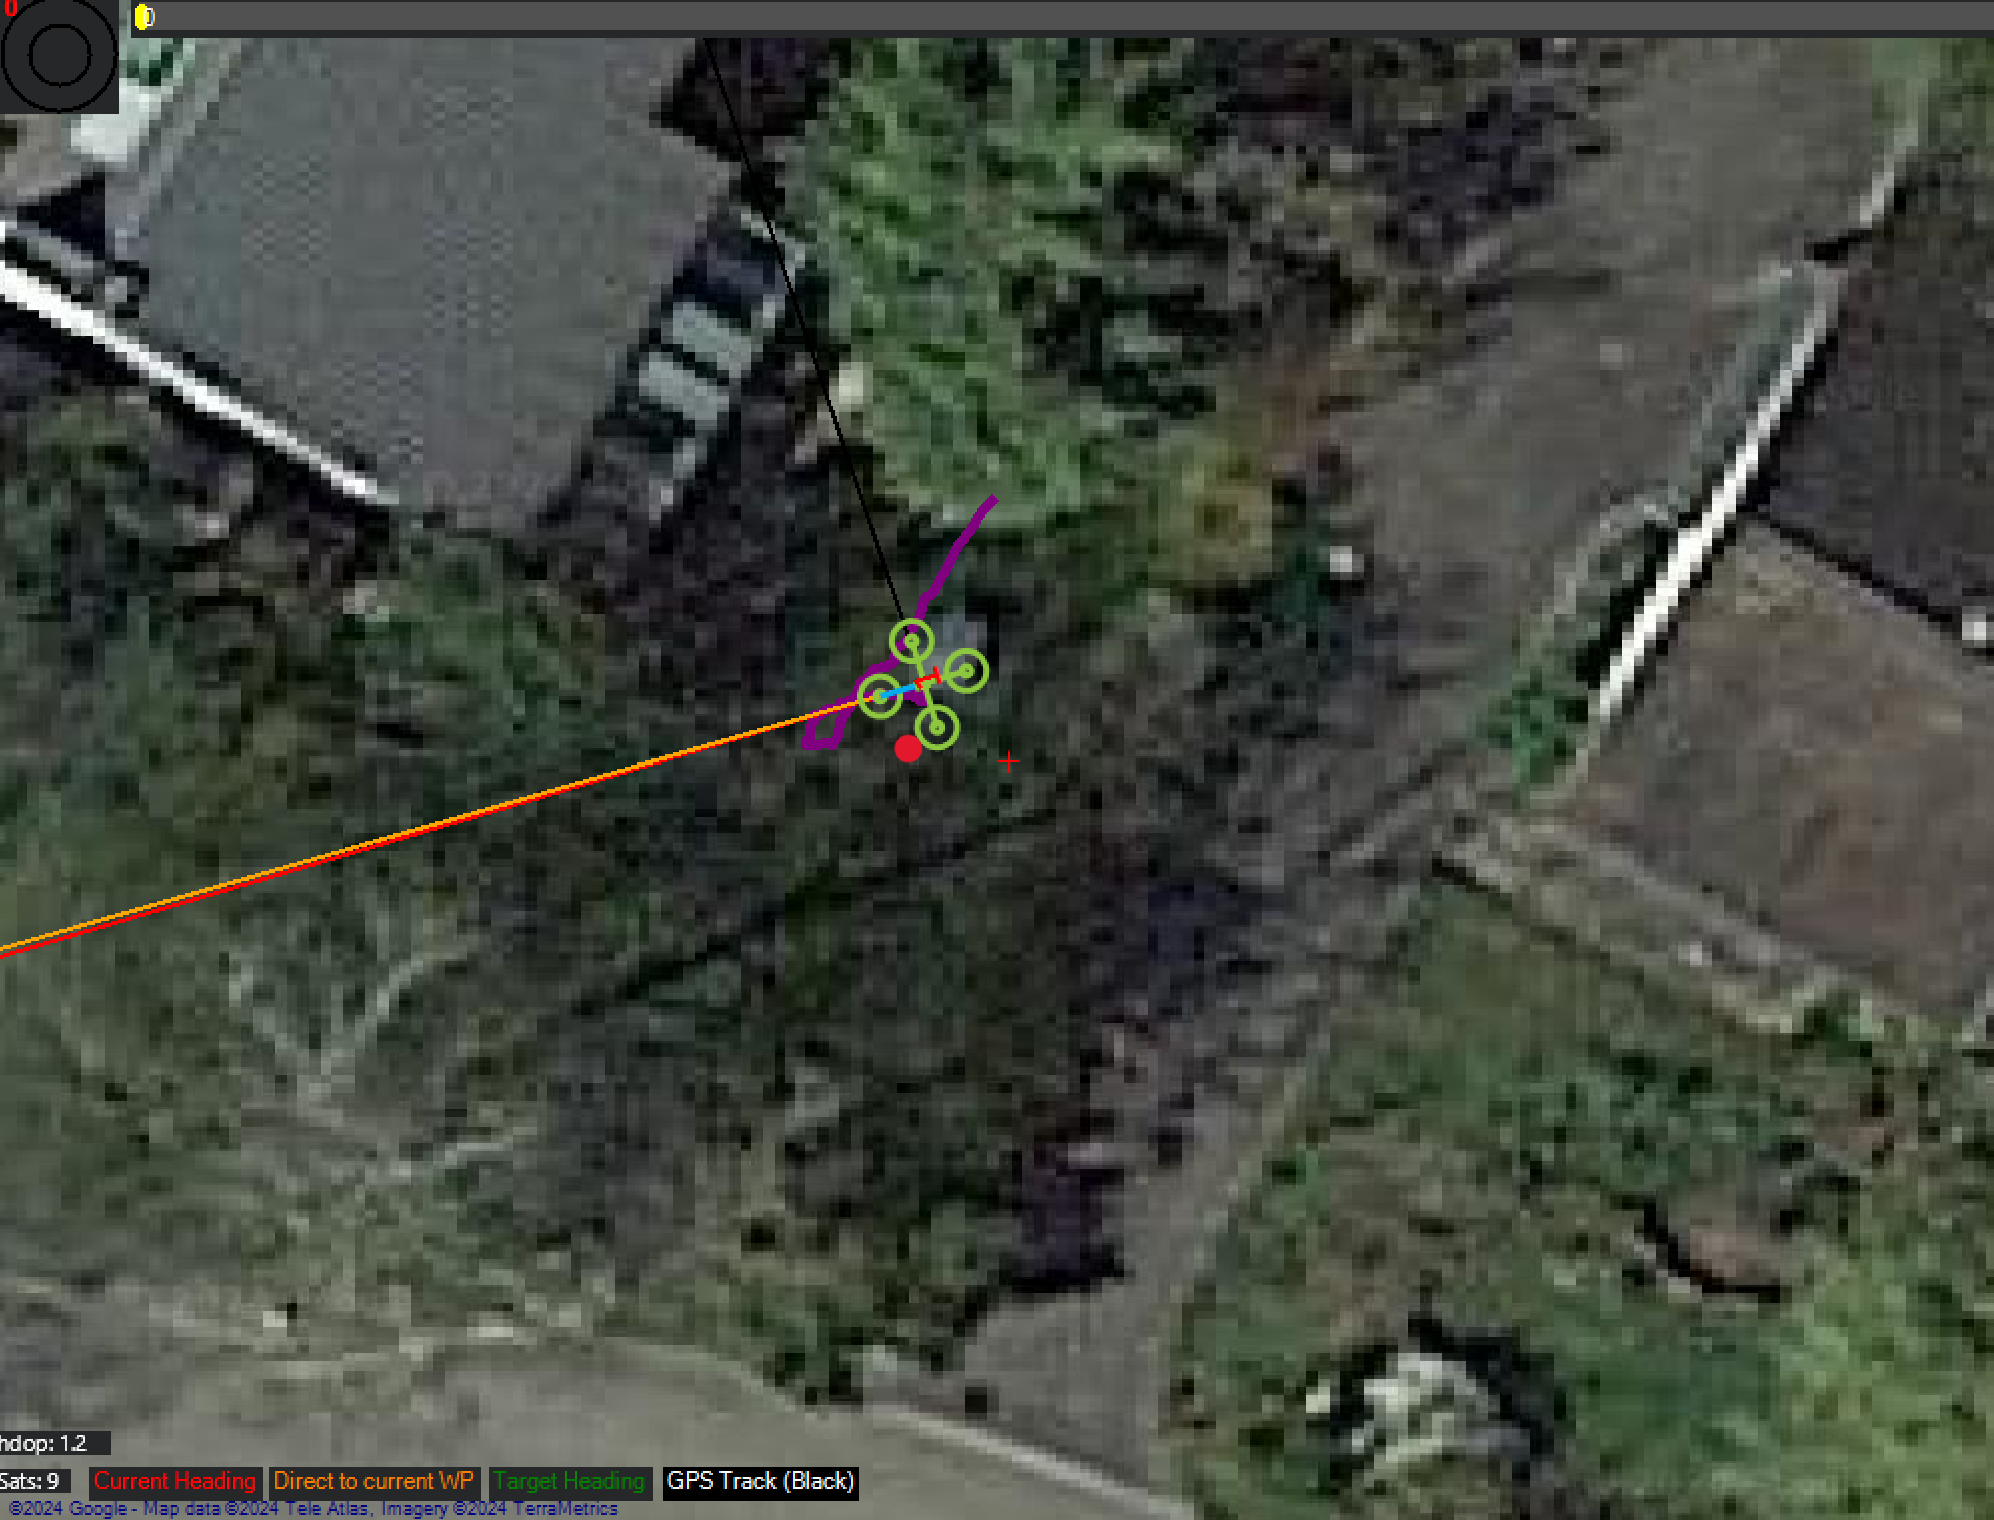
\includegraphics[scale=0.2]{pictures/GPS_Outsidewithdot}
	\caption{\gls{GPS} outside}
	\label{fig:gpsoutside}
\end{figure}
	
	

	 
	\subsubsection{Receiver/Transmitter}
	To establish the connection between the receiver and radio the ExpressLRS page needs to be followed \cite{expresslrsorg}. It required changing the \lstinline|Serial6_Protocol| to 23 and the \lstinline|RSSI_Type| to 3 so it can be the receiving end. I also changed the \lstinline|RC_Options| to the correct bitmask (\cref{fig:bitmask}).

\begin{figure}[ht]
	\centering
	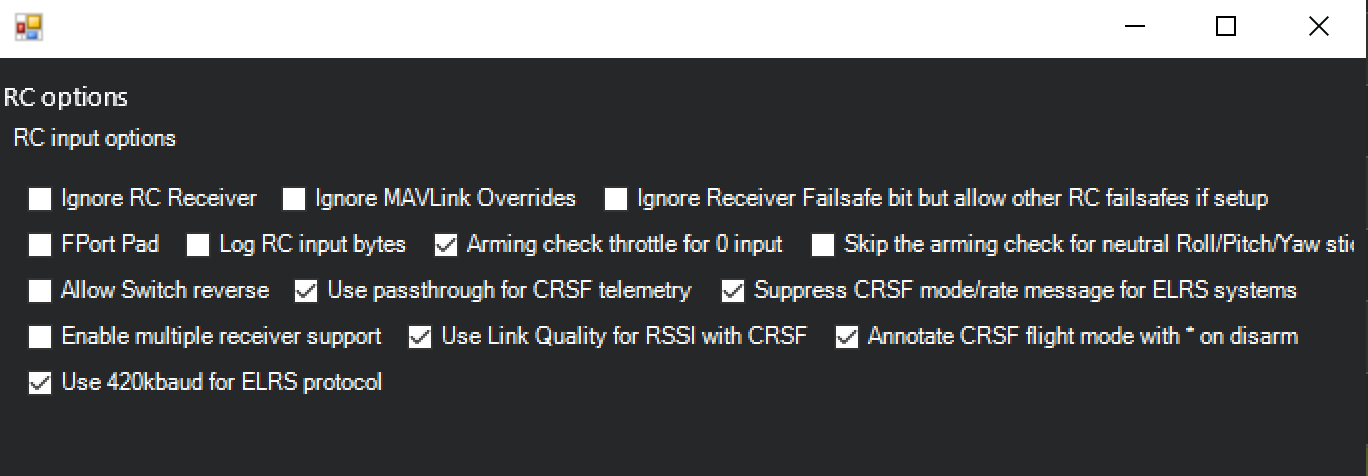
\includegraphics[width=0.7\linewidth]{pictures/bitmask}
	\caption{correct bitmask for ExpressLRS}
	\label{fig:bitmask}
\end{figure}

	The connection between the radio and receiver seemed to be working, because the receiver had a constant blue light. The radio notified that the telemetry recovered after it was lost for a moment. However, it did not yet have a connection to the Fc. There was the possibility to change the Uart6 to the Uart1, which is usually the Uart used for receivers with the Kakute H7, but it would require a JST (a special connector) and more soldering. The solution was found in the Kakute H7 tab in the ArduPilot documentation, in which was written, that for a CRSF\footnote{Even though it is a ELRS receiver it has the same interface as CRSF receivers} interface the parameter \lstinline|Brd_Alt_Config| needs to be set to 1. \lstinline|Brd_Alt_Config| is a Fc specific parameter, this is also the reason why it did not come up in the ExpressLRS page or the ArduPilot documentation. 

	\subsubsection{Battery}
	The battery was rather straightforward. The smoke stopper did not light up when plugging the battery in. In the beginning the battery was not recognized by the \gls{Fc}, but this was solved by changing the parameter \lstinline|Batt_Monitor| to 4. After which the voltage and amperage showed up in \gls{MP}.

	\subsubsection{Motor Test}
	The motor test worked correct after assigning the right position to the motors. Which needed to be done, as I am using the ports M5-M8, instead of the M1-M4. Additionally the parameter \lstinline|Mot_PWM_Type| needs to be set to \mydshot 600. \Gls{DShot} is the digital protocol for communication between the \gls{Fc} and \gls{ESC}. The motors began to beep after a certain time, due to the beacon delay. This will be turned of later. This was also the first time the \gls{ESC} had power, because that a new error appeared called 'battery failsafe'. This is caused by an unstable connection between the \gls{ESC} and the \gls{Fc}, which causes the \gls{Fc} to take the USB cable from the computer as power source and has through too little power to spin the motors, as they need a higher voltage than provided by the computer.
	
	\subsubsection{Compass Calibration}
	The compass calibration needs a good \gls{GPS} lock. However, even with a good lock, relaxed fitness\footnote{The fitness can be in four different states very strict, strict, default and relaxed. The stricter the fitness is the longer the calibration takes.}, and \lstinline|Compass_Orient| set to 6, as recommended by the Holybro docs, it still failed \cite{HolybroDocs}. Large metal parts could again influence the calibration, but there were none in the vicinity of the compass. To temporarily do the calibration the large vehicle MagCal\footnote{The compass calibration is done by rotating the copter in the air. However, this is not really an option for larger vehicles, to calibrate them the large vehicle MagCal is used, by just putting in the direction the compass is facing.} can be done. However, this mostly takes away the prearm message. It is strongly discouraged by the ArduPilot documentation, because it can look as if it is correctly configured, but the orientation is incorrect. The best way to calibrate the compass is to put it directly on  top of the \gls{Fc} and then do the calibration.

	\subsubsection{Road to First Flight}
	The first step to flying is to arm the drone.
	\begin{Explanation}[to arm]
		\item To arm a drone means that the motors begin to spin without producing enough thrust to lift the drone from the ground. It is a safety measure, to prevent the motors from accidentally spinning, when handling the drone.
	\end{Explanation}
	For that a switch on the radio needs to be assigned to arming and disarming. In my configuration the switch five is used. In order for it to work the parameter \lstinline|RC5_Option| is set to 153, which means to arm the drone when the switch number 5 is flicked. To test the drone on the bench inside there will be many prearm errors to ignore the parameter \lstinline|Arming_Check| is disabled and more importantly the geofence, which still blocks the arming when \lstinline|Arming_Check| is disabled. 
	% TODO change the sentence above, if not look that no new paragraph is created here
	After this when flicking the switch 5 the motors will arm and spin\footnote{A battery needs to be connected.}. From my experience it is really important to tie down every cable or antenna before arming the drone with propellers, else they might just be cut or teared off. This will cause a new prearm error to appear called 'crashdump bin detected'. Which is a file that is created when the drone crashes and can be used to analyze the crashes your drone has had. As long as it is tested on the bench, it should not be a problem and can be deleted by flashing new firmware onto the drone \cite{blogcrashdump}. This time however not via STM32CubeProgrammer, but directly over \gls{MP}. Additionally some of the motors need to be reversed for the X-configuration of the drone, seen in \cref{fig:quadx}. To reverse them the reverse button in \gls{MP} does not work. The BLHeliSuite32 software is needed and the parameter \lstinline|Servo_BLh_Auto| is set to 1 which enables a pass through from the \gls{ESC} through the \gls{Fc}. In the software, one can change the motor spinning direction. It is also advisable to turn off beacon delay, at least for now, or else the motors will beep after ten minutes of being idle.
	\begin{Explanation}[beacon delay]
		\item The beeping of the beacon delay is used to located a crashed drone. If the drone has lost the contact to the radio it will automatically activate after a certain amount of time.
	\end{Explanation}
	
\begin{figure}[ht]
	\centering
	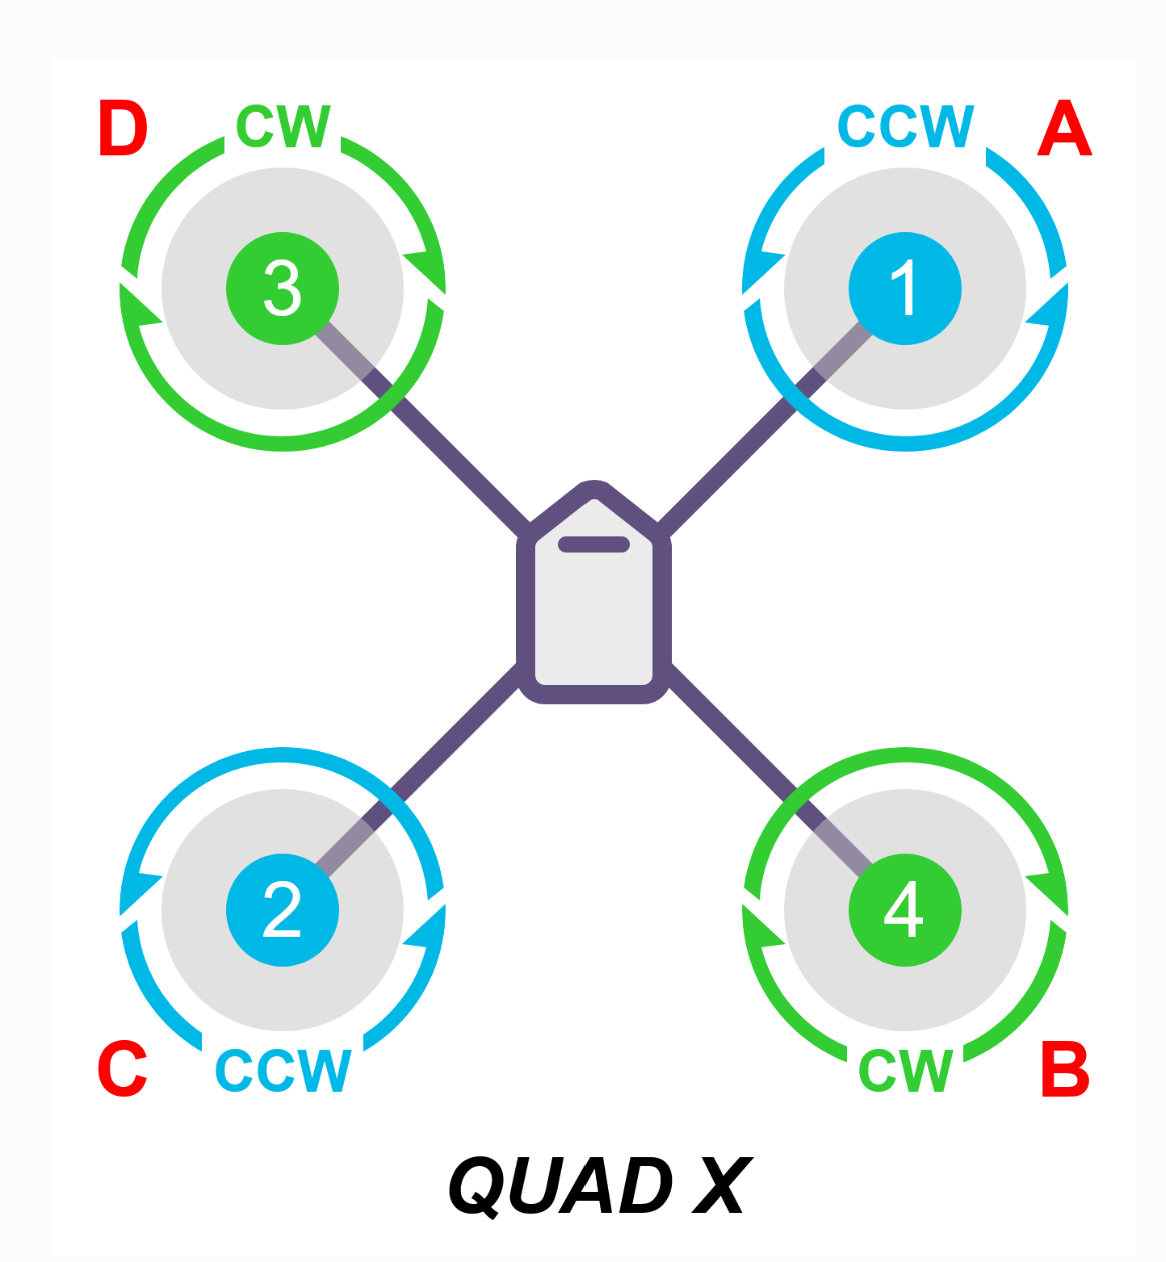
\includegraphics[scale=0.4]{pictures/quadx}
	\caption{Motor turning directions}
	\label{fig:quadx}
\end{figure}
	%TODO fix this picture placement
	In the first test flight the drone was shaking violently, which is also known as wobbling. This caused the drone to crash  into the ground. Reasons for this behavior can be loosely fastened parts, imbalanced propellers, or wrong parameters used for the \gls{PID} controller \cite{dronewobblevideo}. In this case those parameters were for a 9-inch drone and not a 5-inch. The parameters can be adjusted via the initial tuning parameter. After this the drone flew fine, except that the sticks of the radio controller needed to be reversed, because when one pulled the stick left the drone flew to the right. This can be done using the \lstinline|RC2_Reversed| parameter.

	\begin{Explanation}[{{proportional, integral, derivative (PID)}}]
		\item The three parameters are used as weights for the three parts (\gls{PID}) of the error function.
	\end{Explanation}
	
	\subsection{Companion Computer}\label{companion computer}
	The following section is rather technical and can be used as a reference to reproduce the combination of the Kakute H7 and a RaspberryPi working together using Dronekit python.
	\subsubsection{RaspberryPi Setup}
	
	To let the drone fly on its own a companion computer is needed. Due to the \gls{Fc} does not having enough power to process more complex operations such as autonomous flight.
	
	Choosing the RaspberryPi instead of another companion computer is advisable, due to it being the most popular in drone projects.
	% TODO guides ??
	
	The RaspberryPi is not shipped with a microSD card and through that also not with the \gls{OS}. To download the \gls{OS}, the RaspberryPi Imager is used. Through the imager it is possible to create an account for the RaspberryPi,  configure the WiFi and the possibility for a \gls{SSH} connection. 

	
	To see a desktop instead of only a command line based interface with an \gls{SSH} a \gls{VNC} is used. In this case the recommended option was RealVNC viewer a widely used \gls{VNC}. To be able to use RealVNC, RealVNC server needs to be installed over the terminal via \lstinline|sudo apt-get realvnc-vnc-server| \cite{ionisvnctutorial}\footnote{\lstinline|realvnc-vnc-viewer| is only required if you want to see a VNC from the RaspberryPi}.
	
	\subsubsection{MAVProxy Installation}
	The following was based on the MAVProxy Documentation from the ArduPilot website  \cite{MavProxydocs}.
	
	Firstly all the necessary packages need to be installed through the \lstinline|sudo apt-get install| command. 
	\begin{lstlisting}
		sudo apt-get install python3-dev python3-opencv python3-wxgtk4.0 python3-pip python3-matplotlib python3-lxml python3-pygame
		pip3 install PyYAML
	\end{lstlisting}

	What is not said in the MAVProxy Documentation, is that you need a \gls{venv} and cannot download it without one or the error; \lstinline|error: externally-managed-environment| pops up. To get around this issue you need to create and activate a \gls{venv}.
	\begin{lstlisting}
		python3 -m venv mavproxy-env
		source mavproxy-env/bin/activate
		pip install MAVProxy
	\end{lstlisting} 
	
	
	To connect the drone over MAVProxy it needs to know how the \gls{Fc} is connected to the RaspberryPi. The command \lstinline!dmesg | tail! will provide the information, as seen in \cref{fig:usbrasppiconectrectangle}.

\begin{figure}[th]
	\centering
	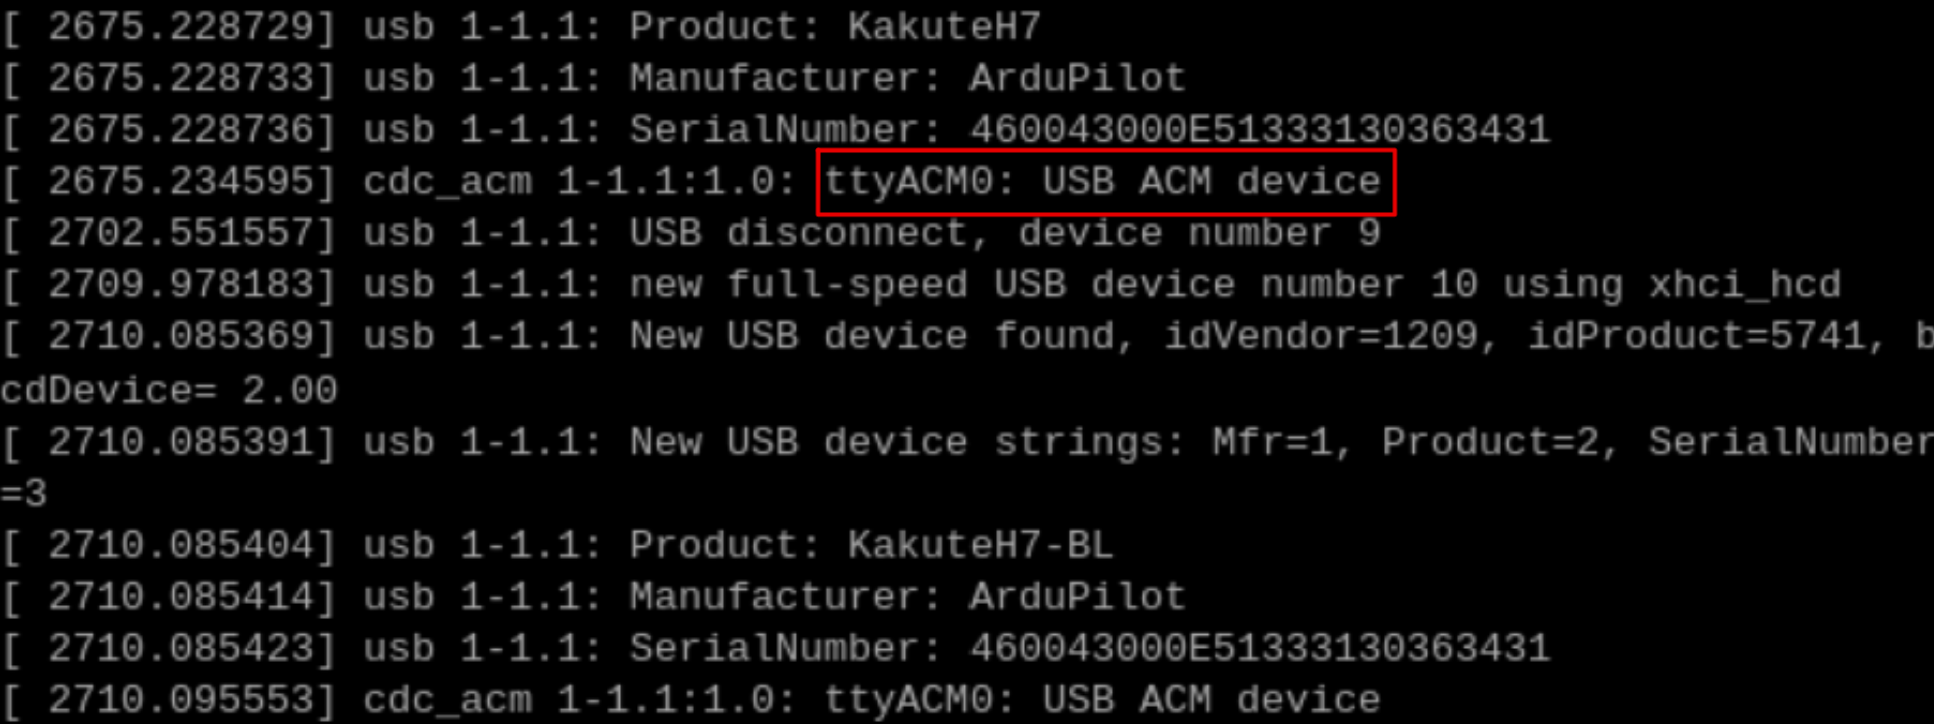
\includegraphics[width=0.7\linewidth]{pictures/USBRaspPiconect_rectangle}
	\caption{output from \lstinline!dmesg | tail!}
	\label{fig:usbrasppiconectrectangle}
\end{figure}

	
	The command \lstinline|mavproxy.py --master=/dev/ttyACM0 --baudrate 115200 --aircraft MyCopter|, is used to connect over MavProxy, an error will appear if \lstinline|\ttyUSB0| instead of \lstinline|\ttyACM0| is utilized. If the RaspberryPi is connected over the serial ports, \lstinline|\serial0| is used instead of \lstinline|\ttyACM0|. The baudrate can also vary, in this case it is 921600. The RaspberryPi will not have another power source except over the \gls{Fc}, the 5+ V pin on the RaspberryPi needs to be connected to a 5 volt pin on the \gls{Fc} and additionally a ground pin. There can be a low voltage warning, even though the RaspberryPi is not receiving enough power, it is sufficient to run Dronekit python code. In addition the \lstinline|Serial3_Protocol| needs to be changed to 2 for the MAVLink protocol.
	% TODO look at the sentence: The RaspberryPi will not have another power source except....
	
	When connected to the \gls{Fc} you can use simple commands to change the parameters, as \lstinline|param set arming_check 0|, or to arm the copter with \lstinline|arm throttle|.
	
	\subsubsection{Dronekit}
	It first needs to be mentioned that the Dronekit python software is not maintained very well, as it is stated in the Github repository \cite{dronekitgithub}. The following is still mostly based on the Dronekit Documentation \cite{dronekitdocs}.
	
	% TODO add flowchart of the code for what is planned
	
	First the Dronekit library needs to be installed in the \gls{venv} with \lstinline|pip install dronekit|. To create a file in the \gls{venv} over the terminal \lstinline|nano dronekittest.py| is used. It is noteworthy not to use the same name as the library itself, because python will confuse it. In the created document one then can connect the RaspberryPi to the \gls{Fc} as can be seen in \cref{lst:listing-connection}.
	\begin{lstlisting}[language=Python, style=myPython, caption=Python DroneKit Example, label=lst:listing-connection]
		from dronekit import connect

		vehicle = connect('/dev/serial0', baud=912600, wait_ready=True)
	\end{lstlisting}
	
	However this will cause an attribute error, as one can see in \cref{lst:attributeerror} 
	\begin{lstlisting}[label=lst:attributeerror, caption={AttributeError after connecting}]
		dronekit/__init__.py" , line 2689, in <module>
		class Parameters(collections.MutableMapping, HasObservers):
		^^^^^^^^^^^^^^^^^^^^^^^^^^
		AttributeError: module 'collections' has no attribute 'MutableMapping'
\end{lstlisting}
	The source of the error is that in python 3.10 the abstract base class, MutapleMapping, was moved from collections to collections.abc. This needs to be changed (\cref{changed line}) in the dronekit source code. Which can be accessed with the the command \cref{sourcecode}\footnote{If it would not be open source, the change(\cref{changed line}) would not be possible}.
	
	\begin{lstlisting}[caption= accessing source code, label=sourcecode]
nano /home/EduPi/mavproxy-env/lib/python3.11/site-packages/dronekit/__init__.py
\end{lstlisting}

	\begin{lstlisting}[caption={changed line in source code (change marked in green)}, label=changed line, language=python, style=myPython, literate={.abc}{{\color{Green}.abc}}4]
		class Parameters(collections.abc.MutableMapping, HasObservers):
	\end{lstlisting}
	
	After this the program worked flawlessly and it was able to give information from the \gls{Fc} over the terminal. As shown with the example \cref{lst:listing-autopilot}, which 
	
	\begin{lstlisting}[language=python, caption={information retrieval}, label=lst:listing-autopilot, style=myPython]
		print( "Autopilot version: %s" %vehicle.version)
	\end{lstlisting}
	\begin{lstlisting}[caption= output from \cref{lst:listing-autopilot}]
		Autopilot version: APM:Copter-4.5.7
	\end{lstlisting}

	The main problem of the outdated Dronekit python library is, that the function \lstinline|vehicle.channels|, which should read the channel values from the radio controller, is returning none instead of values between 900 and 2100. This is a long-known issue and to circumvent it a decorator is used \cite{rcchannelissue}. 

	\begin{Explanation}[Decorator]
		\item A decorator is a function that modifies the behavior of a function or a class \cite{decorator}.
	\end{Explanation} 
	
	\begin{lstlisting}[language=python, style=myPython, label=lst:decorator, caption={decorator for channel values}]
		@vehicle.on_message("RC_CHANNELS")
		def rc_channel_listener(vehicle, name, message):
			global latest_rc_channels
			latest_rc_channels = message
		
		def get_rc_channel_value(channel_number):
			global latest_rc_channels
			if latest_rc_channels is None:
				return None
			channel_value = getattr(latest_rc_channels, f"chan{channel_number}_raw", None)
			return channel_value
		
	\end{lstlisting}
	The decorator in \cref{lst:decorator} is already predefined in the Dronekit library. When calling it with \lstinline|@vehicle.on_message("RC_CHANNELS)| (line 1 \cref{lst:decorator}) and saving it to the global variable \lstinline|latest_rc_channels| (line 4 \cref{lst:decorator}) as a dictionary (\cref{lst:message}).
	
	\begin{lstlisting}[label=lst:message, caption={output from decorator in \cref{lst:decorator}\protect\footnote{}}]
		chan{i}_raw : x
	\end{lstlisting}
	\footnotetext{With i being the channel number and x the value the channel receives form the radiocontroler}
	
	The location is straight-forward. There is a home location that is set every time the drone is armed. In addition there is also local frame generated with it, which takes over the coordinates for north and south, but sets the height to 0 at the starting point. The home location could also be newly set via a MAVlink command. To access any given location local or global can be done over \lstinline|vehicle.location.global_frame|\footnote{"vehicle" is the connection to the \gls{Fc} from \cref{lst:listing-connection}}. This will have a list output \lstinline|[longitude, latitude, altitude]|, to access the longitude a \lstinline|.lon| is added after the \lstinline|_frame| from before\footnote{\lstinline|.lat| for the latitude and \lstinline|.alt| for the altitude}.
	
	I personally added the \lstinline|log()| function to be able to troubleshoot what went wrong in the testflight, can be seen in \cref{lst:logfunciton}. On line 2 the correct file is defined, which is then opened in append mode in line 3. Line 4 writes the given content into the file and line 5 closes the file again.
	
	\begin{lstlisting}[style=myPython, caption={log function}, label=lst:logfunciton]
		def log(content):
			p = pathlib.Path(__file__).with_name('log.txt')
			o = p.open(mode="a")
			o.write("\n"+ str(datetime.now())+"	" +str(content))
			o.close()
	\end{lstlisting}
	
	The desired coordinates for the drone to fly to are taken from a .tex file in the format \lstinline|X;Y;Z| in meters and need to be converted into degrees. This is done by the code from \cref{lst:coordinatesconversion}.
	
	\begin{lstlisting}[style=myPython, caption= coordinate conversion, label=lst:coordinatesconversion]
		earth_radius = 6378137.0
		
		changeX = home_location.lat + math.degrees(float(X[i]) / earth_radius)
		changeY = home_location.lon + math.degrees(float(Y[i]) / (earth_radius * math.cos(math.radians(home_location.lat))))
		changeZ = home_location.alt + float(Z[i])
		
	\end{lstlisting}
	
	To fly to a certain coordinate the \lstinline|vehicle.simple_takeoff| and the \lstinline|vehicle.simple_goto| functions are used. However, with the standard parameters from ArduPilot this will not work, because the parameters bitmask of  \lstinline|Brd_Safetyoption| is set to be active even when \lstinline|Brd_safety_deflt| is deactivated. 
	This will not let anything, except the channels defined in \lstinline|Brd_Safety_Mask|, go through to the \gls{ESC}. Hence both of them need to be deactivated by the code, as demonstrated in \cref{lst:deactivation}
	\begin{lstlisting}[caption={deactivation of parameters}\protect\footnote{}, style=myPython, label=lst:deactivation]
		vehicle.parameters["BRD_SAFETYOPTION"] = 0
	\end{lstlisting}\footnotetext{This can be done with any parameter, by putting it into the place of \lstinline|Brd_Safetyoption|.}
	
	Something that needs to be looked out for when flying low over the ground is that there is a low \gls{VDOP}, because it is not one of the prearm messages that would hinder the drone from taking off. 
	
	\begin{Explanation}[horizontal and vertical dillution of precision (HDOP/VDOP)]
		\item The \gls{HDOP} or \gls{VDOP} refers to the dillution of the precision of the \gls{GPS}. The values are not in meters and range from under 1 (ideal) up to over 20 (poor). 
	\end{Explanation}
	
	\section{Results}

	The various testflights showed promising results. The drone followed the path from the coordinates.txt file, which was the main goal of this Matura paper. The different trials showed also, how much one or two parameters already influence the capability of the drone to fly. 
	
	Another challenge was integrating the different software components, which are not transparent and sometimes outdated. The software components often conflicted during drone takeoff, with one allowing flight while another prevented it\footnote{The prevention was the one with the upper hand.}.

	This Matura paper also shows how important a log file is for an autonomous system, because once the system takes  control, it is impossible to know what is happening and without the data provided by a log file one can also not improve the system.
	
	
	\section{Discussion and Outlook}
	 It should be noted that the built drone is only a proof of concept and requires further testing and tuning to reach full maturity. Additionally, a (infrared) camera can be added to the RaspberryPi. Due to the nature of the RaspberryPi being a fully functioning computer, unlike an Arduino, the pictures taken by the camera could be processed directly on board for tasks such as image recognition. This would be straight-forward, because it is already integrated into the in RaspberryPi.
	
	\section{Conclusion}
	\newpage
	\renewcommand{\thesubsection}{\Alph{subsection}}
	\counterwithin{figure}{subsection}
	\counterwithin{table}{subsection}
	\pagebreak
	\appendix
	\section{Appendices}
	

	\printbibliography
	
	\newpage
	\listoffigures
	% TODO mdight sort them by author...

	\newpage
	\printglossary[type=\acronymtype]
	\newpage
	\subsection{List of Parts}
	\subsubsection{Physical Parts}
	\begin{itemize}
		\item \gls{Fc}:		Kakute H7 v1.3 (MPU6000) \cite{KakuteH7}
		\item \gls{ESC}: 	Tekko32 F4 Metal 4in1 65A ESC (AM32) \cite{Tekko32}
		\item \gls{GPS}: 	Micro M10 GPS \cite{m10gps}
		\item 4 Motors: 	XING-E Pro 2207 2450KV \cite{xingepro}
		\item Propellers: 	Foxeer Donut 5145 Props \cite{toroidal} or HQProp 5X4.3X3V1S \cite{hqprops}
		\item Battery: 		Tattu 2000mAh 4S 120C 14.8V R-Line Version 3.0 \cite{tattu}
		\item Receiver: 	RP4TD ExpressLRS 2.4GHz True Diversity Receiver \cite{radiomasterreceiver}
		\item Radio: 		Boxer Radio Controller (M2) \cite{radiomasterboxer}
		\item RaspberryPi:	Raspberry Pi 4 Model B - 2GB \cite{raspberrypi}
		\item Frame:		TBS Source One V5.1 5inch \cite{frame}
		\item Additional Screws: 4x M3x20, 4x M3x30 (for the \gls{Fc}/\gls{ESC} stack), 4x M3x40
	\end{itemize}
	\subsubsection{Non-Physical Parts}
	\begin{itemize}
		\item RaspberryPi Mount: 	\url{https://github.com/pythonnoob9903/MA-project/tree/main/RaspberryPi%20Mount}
		\item Code and Coordinates\footnote{Found as dronekittest.py, coordinates.py, and coordinates.txt}:  \url{https://github.com/pythonnoob9903/MA-project/tree/main}
	\end{itemize}
	
\end{document}
